\documentclass[12pt,a4paper,utf8x]{report}
\usepackage [frenchb]{babel}

%\usepackage{ucs}
%\usepackage{pgfgantt}
\usepackage{graphicx}
\usepackage{caption}
\usepackage[utf8x]{inputenc}
\usepackage{multicol}
\usepackage{url} % Pour avoir de belles url
\usepackage {geometry}
%\usepackage {listings} %Pour mettre du code source 
\usepackage{verbatim}
\usepackage{lscape} % Pour pouvoir passer en paysage
\usepackage{geometry}
\usepackage{pdflscape}
\usepackage{colortbl}
\usepackage[strings]{underscore}
\geometry{left=2.5cm,right=2.5cm,vmargin=2cm}
\usepackage[pdftex,bookmarks = true,bookmarksnumbered = true,pdfpagemode = None,pdfstartview = FitH,pdfpagelayout = OneColumn,colorlinks=true,linkcolor=black,urlcolor=blue,citecolor=blue,pdfborder = {0 0 0}]{hyperref}


%chapitre---------------------------------------------------------------------
 
%%%% debut macro pour enlever le nom chapitre %%%%
\makeatletter
\def\@makechapterhead#1{%
  \vspace*{50\p@}%
  {\parindent \z@ \raggedright \normalfont
    \interlinepenalty\@M
    \ifnum \c@secnumdepth >\m@ne
        \Huge\bfseries \thechapter\quad
    \fi
    \Huge \bfseries #1\par\nobreak
    \vskip 40\p@
  }}

\def\@makeschapterhead#1{%
  \vspace*{50\p@}%
  {\parindent \z@ \raggedright
    \normalfont
    \interlinepenalty\@M
    \Huge \bfseries  #1\par\nobreak
    \vskip 40\p@
  }}
\makeatother
%%%% fin macro %%%% 

\begin{document}

%\begin{titlepage}
%\begin{flushright}
%   	
\includegraphics[scale=0.30]{univorleans.png}\\ 
%   	   	Département Informatique
%\end{flushright}
%\vspace{30mm}
%\begin{center}
%\huge{Mémoire intermédiaire \\Travaux d'étude et de recherche }\\
%\vspace{8mm}
%\large{Sujet : Android au pays des liseuses}\\
%\vspace{3mm}
%\large{Proposé et encadré par : Ollinger Nicolas}
%\vspace{3mm}
%\large{\\Réaliser par :}\\
%\large{Fontorbe Jordan, Guillaume Arthur, Monediere Tristan, \\Rubagotti Joris}\\
%\end{center}
%\begin{figure}[b!]
%\begin{flushright}
%~~\\ ~~\\ ~~\\ ~~\\ ~~\\ ~~\\ ~~\\
%\large{Année : 2012-2013}
%\end{flushright}
%\end{figure}
%\end{titlepage}

%\tableofcontents
%\clearpage

\section {utilitaire}
\subsection{montage du système de fichier de la liseuse}
	%copie des fichiers (montage de la carte sd ...)
	mount -o loop -t ext4 [PATH_to_sd_card]/Os firmware/files/update.img  [dossier_de_montage]


\section{Compilation du module g_ether}
	%configuration de la compilation(cf lien)
	\subsection{configuration}
		On utilise le compilateur gcc 4.4.3 fournit avec le ndk android.
		(bien penser à avoir le ndk android dans son PATH).
		configuration du ndk : 
		\begin{verbatim}
			export CROSS_COMPILE=arm-eabi-
			export PATH=[PATH_to_ndk]/linux-x86/toolchain/arm-eabi-4.4.3/bin
			export SUBARCH=arm
			export ARCH=arm
		\end{verbatim}
		mise en place de la configuration officielle du kernel : 
		\begin{verbatim}
			zcat [PATH_to_terkit]/nopid/livedata/config.gz >[PATH_to_terkit]/sony/linux-2.6.35.3/.config
		\end{verbatim}
		Ensuite il faut faire un make menuconfig et éditer  : 
			\begin{itemize}
				%certains : 
				\item  Device drivers $>$ usb support $>$ usb gadget support $>$ Ethernet gadget -$>$ $<$M$>$ with RNDIS support
				%peut-être useless
				\item Device drivers $>$ usb support $>$ usb gadget support $>$ CDC composite device
			\end{itemize}

Pour compiler : "make modules"
		
		Ensuite il faut copier les fichiers g_ether.ko et g_cdc.ko sur "/lib/modules/[version]/kernel/drivers/usb/gadget" (système de fichier de la liseuse)
	
	%installation des modules (modification des scripts)
\subsection{installation des modules}	
	Les deux modules g_serial et g_ether ne peuvent pas être lancés en même temps, il faut donc modifier sur la liseuse le fichier "/etc/rc.d/rc.local" de manière à ce qu'il coupe le module g_serial et lance g_ether à la place.
	%ajout code rc.local
	\begin{verbatim}
		echo "modprobe -r g_serial" > /initrd/mnt/sd/test/log
		#desactivation de g_serial
		modprobe -r g_serial 2>> /initrd/mnt/sd/test/log
		echo "modprobe g_ether" >> /initrd/mnt/sd/test/log
		#activiation de g_ether
		modprobe g_ether host_addr=00:00:00:00:00:01 dev_addr=00:00:00:00:00:02 2>> /initrd/mnt/sd/test/log
		#on demarre l'interface
		ifconfig usb0 up
	\end{verbatim}
	Les options host_addr et dev_addr permettent à la liseuse d'affecter son adresse mac mais aussi celle du pc sur lequel elle est connecté (host), cela permet de ne pas avoir à refaire la configuration réseau à chaque branchement.	
	%connection depuis le pc
	Pour se connecter depuis le pc penser à vérifier que le module usbnet est bien activé	
	Un interface réseau devrait apparaître, il faut la configurer sur le réseau 192.168.1.0/24 (la liseuse est configurer sur l'adresse 192.168.1.1/24)
	%
	%le fichier log permet ... de faire des logs [captain obvious]
	%modification des scripts de demarrage
	
%\section[Intruduction]{Introduction au domaine}


\subsection[E-Ink]{Technologie E-Ink}
\begin{frame}{Technologie E-Ink}
	%% A compléter par Arthur
\end{frame}


\subsection[Sony PRS-T1]{Liseuse Sony PRS-T1}

\begin{frame}{Caractéristiques principales} %% Liseuse en générale
	\begin{block}{Caractéristiques Sony PRS-T1}
		\begin{itemize}
			\item Processeur iMX508
			\item Écran E-Ink 6 pouces
			\item Résolution jusqu'à 16 niveaux de gris
			\item Interfaces USB
			\item WiFi
			\item Mémoire : 2Go (extensible par microSD)
		\end{itemize}
	\end{block}
\end{frame}

\begin{frame}{Processeur iMX508} %% partie iMX508
	\begin{block}{iMX508}
	\begin{itemize}
		\item{Développé par Freescale}
		\item{Architecture ARM Cortex A8}
		\item{Faible consommation d'énergie}
		\item{Bonnes performances}
		\item{Contrôleur d'écran intégré}
	\end{itemize}
	\end{block}
\end{frame}

\begin{frame}{Modules}
	\begin{block}{EPDC (Electrophoretic Display Controller)}
		\begin{itemize}
			\item{Dirige les signaux (waveform)}
			\item{Mise à jour partielle ou totale}
		\end{itemize}
	\end{block}
	\begin{block}{ePXP (enhanced Pixel Pipeline}
		\begin{itemize}
			\item Transparence
			\item Rotation d'image
			\item Agrandissement / Réduction d'image
		\end{itemize}
	\end{block}
\end{frame}

\begin{frame}{Architecture du processeur iMX508} %% Schéma
	\begin{figure}
		\begin{center}
			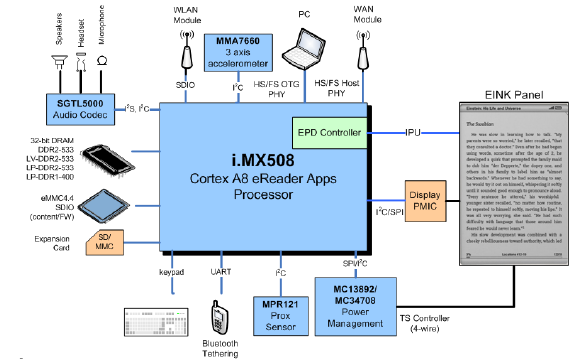
\includegraphics[scale=0.65]{iMX508.png}
		\end{center}
	\end{figure}
\end{frame}

\begin{frame}{Hack de la liseuse}
	\begin{block}{Mise à jour du firmware}
		\begin{itemize}
			\item Nécessite les clés privés de Sony
			\item Accès total à la liseuse
			\item Risque d'endommager la liseuse
		\end{itemize}
	\end{block}
	\begin{block}{Mode Recovery}
		\begin{itemize}
			\item Nécessite la recompilation du noyau
			\item Modifications sans risques
		\end{itemize}
	\end{block}
\end{frame}

%\chapter{Analyse de l'existant}
%\chapter{Besoins non fonctionnels}
\section{Hacks de la PRS-T1}

La PRS-T1 étant fermé, il nous est impossible dans sa configuration de base de pouvoir y ajouter la mise à jour 
de l'affichage depuis une machine hôte.
Plusieurs méthode existent pour débloquer la liseuse : 

\subsubsection{Mise a jour du firmware}

La méthode la plus répandues pour débloquer la liseuse consiste à faire une mise à jour du firmware.
La liseuse n'acceptant que les mises à jour signée par Sony. Les clefs privées de cette signature étant connues des hackers (elles sont stoquées dans la liseuse pour la vérification).

Plusieurs firmware modifié existe déjà pour mettre à jour la liseuse, c'est derniers débloque complètement la liseuse tout en gardant les logiciels Sony pré-installé.

Cette méthode dispose donc de plusieurs avantages : 
	\begin{itemize}
		\item permet un accès total a la liseuse (installation d'application Android, ...)
		\item on conserve les fonctions normale de la liseuse (logiciel de lecture Sony)
	\end{itemize}
Cependant le fait de modifier le firmware interne de la liseuse comporte certains risques : 
	\begin{itemize}
		\item risque de rendre la liseuse inutilisable
		\item perte de la garantie constructeur
	\end{itemize}

Étant donné que la PRS-T1 est un prêt de M. Ollinger cette méthode de hack comporte trop de risques.

\subsubsection{Utilisation du mode Recovery}

Une autre méthode de hack consiste à utiliser le mode recovery de la liseuse.
Ce mode permet normalement de récupérer la liseuse suite à un problème.
Pour entrer en mode recovery la liseuse a besoin d'un  système de fichier de récupération.
Ce dernier pouvant être situé sur une carte mémoire externe.

Cette méthode réduits les risques encouru lors de la manipulation car un simple redémarrage de la liseuse, 
suffit pour revenir au système de base.

les caractéristiques de cette méthodes sont  : 
%Les avantages de cette méthodes sont : 
\begin{itemize}
	\renewcommand{\labelitemi}{$\bullet$}
	\item Avantages : 
	\begin{itemize}
		\item risque minime pour la liseuse
		\item permet des modifications importante (car on fait nous même le système à partir des sources du noyau fournit par Sony)%un peu long non ?
	\end{itemize}
	\item désavantages : 
		\begin{itemize}
			\item nécessite un pc hôte pour la mise en place du système (nécessitent de compiler le noyau)
			\item On repart de zéro donc on n'a pas accès aux application sony (pour la lecture d'Ebook notamment)
			\item nécessite beaucoup de travail car on repart avec uniquement le noyau.
		\end{itemize}
\end{itemize}
\section{Risque}
\subsection{Les Waveformes}
	Le driver permet de redéfinir les fonctions de waveforme du contrôleur.
Cependant le bon fonctionnement des écrans E-Ink dépend fortement de ces fonctions, modifier ces fonctions peut donc entraîner dans le meilleur des cas une différence entre la représentation virtuelle de l'affichage et ce que va réellement afficher l'écran, dans le pire cas cela peu endommager de manière définitive l'écran de la liseuse.

\section{Tests}

La spécificité des liseuses venant de leur écran il faut faire attention a respecter au maximum le comportement de ce dernier pour faire un environnement de développement dédié aux liseuses.

\subsubsection{Taux de rafraîchissement}

Les écrans E-Ink ayant un taux de rafraîchissement assez bas il devient nécessaire de veiller à ne pas le réduire d'avantage.
Pour cela Il va falloir mettre en place un test comparatif entre le rafraîchissement de la liseuse seule et le rafraîchissement avec un ordinateur hôte via VNC.

\subsubsection{Update bloquante}

De la même manière l'ordinateur hôte ne doit pas se comporter de la meme manière qu'avec un écran classique. En effet il serait très facile pour l'hôte de surcharger complètement l'écran en faisant des mises à jour de l'affichage comme il le ferait avec un écran classique. %a véifier un peu tordu
%\chapter{Besoins fonctionnels}

Comme énoncé dans le chapitre 1 de ce document, le but du projet est la réalisation d'un émulateur d'une liseuse avec un écran virtuel fonctionnant comme un écran E-Ink directement sur notre machine ayant pour système d'exploitation Linux. La réalisation de ce projet se découpe en plusieurs parties à réaliser dans un ordre strict afin d'aboutir au résultat final souhaité. Ce plan nous a été proposé par notre encadrant de projet M. OLLINGER. N'ayant pas encore eu le temps de tester les points suivants il se peut que certains des éléments ont été mal interprétés d'où la présence possible d'erreurs. D'autres points peuvent aussi manquer de détails.

\section{Conception d'un client RFB pour la liseuse}

Dans un premier temps il nous faut concevoir un prototype de client permettant de mettre à jour l'écran de la liseuse de test via notre ordinateur.

\subsection{DirectFB}
Pour réaliser cela, il nous a été proposé de travailler avec DirectFB. C'est une bibliothèque libre qui fournit à la fois un accès aux composants matériels graphiques (accélération graphique) ainsi qu'aux périphériques d'entrées, et un systèmes de gestion de fenêtres intégrées avec support de la transparence et de calques multiples. Tout ceci à travers l'interface framebuffer de Linux. Nous devons ajouter la gestion des écrans E-Ink dans DirectFB. 
 
\subsection{Client RFB}
Lorsque DirectFB est prêt à être employé, on travaille ensuite sur le protocole RFB (Remote FrameBuffer) qui est un simple protocole permettant des accès à distance à des interfaces graphiques d'utilisateur. On doit ajouter la gestion des mises à jour de l'affichage pour les écrans de type E-Ink via ioctl. De tous ces éléments, on peut ainsi concevoir un client RFB interagissant sur la liseuse et la conception d'un serveur gérant les mises à jour.
\\Les tests consisteront à essayer de produire des changements d'affichage sur la liseuse grâce à des demandes précises envoyées via l'ordinateur de test et transmis par le serveur de mise à jour. 

\newpage

\section{E-Ink QEMU via VNC}

Dans un second temps, on développe la base de l'émulateur, c'est à dire la mise en place d'une machine virtuelle pouvant reproduire les actions nécessaires au fonctionnement d'un écran E-Ink. Pour réaliser cela, nous travaillons sur QEMU qui permet l'émulation de processeur et de machine virtuelle permettant l'exécution de système d'exploitation. On ajoute la gestion des ioctl à QEMU. Ensuite il faut ajouter à l'option VNC de QEMU l'extension RFB du client de la liseuse.
\\Le test consiste à vérifier si depuis une machine virtuelle QEMU utilisant l'image du noyau Linux de la liseuse de test, on peut via VNC interagir avec la liseuse. 


\section{Liseuse Android sous QEMU}

Après la création de la base de l'émulateur, on intègre à celui-ci un système d'exploitation Android conçu pour fonctionner sur une liseuse. Dans notre cas ça sera la version d'Android présente sur notre liseuse de test SONY PRS-T1.
Pour les tests, on lance l'émulateur muni d'Android et on test le fonctionnement des applications SONY fournies de base avec le système d'exploitation.

\section{Simulation d'écran E-Ink}

Pour finir le développement de l'émulateur, on développe un simulateur d'écran E-Ink reproduisant virtuellement le comportement de celui-ci en y ajoutant des fonctionnalités facilitant les tests telles que choisir une zone précise à mettre à jour sur un écran (utile au debug). Ensuite on intègre celui-ci dans notre émulateur.
\\Les tests consisteraient à réaliser des mini-applications, les lancer sur l'émulateur et vérifier les réactions de notre écran virtuel.


%\chapter{Résultats de tests}
%\begin{landscape}
\chapter{Planning}

\begin{figure}[h!]
\begin{center}

\begin{ganttchart}[y unit title=0.4cm,
y unit chart=0.5cm,
vgrid,hgrid, 
title label anchor/.style={below=-1.6ex},
title left shift=.05,
title right shift=-.05,
title height=1,
bar/.style={fill=gray!50},
incomplete/.style={fill=cyan},
progress label text={},
bar height=0.7,
group right shift=0,
group top shift=.6,
group height=.3,
group peaks={}{}{.2}]{32}
%labels
\gantttitle{Planning}{32} \\
\gantttitle{Février}{8} 
\gantttitle{Mars}{8} 
\gantttitle{Avril}{8} 
\gantttitle{Mai}{8} \\
%tasks
\ganttbar[bar/.style={fill=green, rounded corners=3pt}]{Recherche Doc}{1}{8} \\
\ganttbar[bar/.style={fill=blue, rounded corners=3pt}]{Réunion}{9}{10} \\
\ganttbar[progress=90,bar/.style={fill=orange, rounded corners=3pt}]{Dev DirectFB}{11}{17} \\
\ganttbar[progress=90,bar/.style={fill=orange, rounded corners=3pt}]{Dev Client RFB}{11}{17} \\
\ganttbar[progress=90,bar/.style={fill=orange, rounded corners=3pt}]{Dev Serveur Update}{11}{17} \\
\ganttbar[progress=90,bar/.style={fill=orange, rounded corners=3pt}]{Dev QEMU et VNC}{17}{21} \\
\ganttbar[progress=90,bar/.style={fill=orange, rounded corners=3pt}]{Dev QEMU Liseuse SONY}{18}{22} \\
\ganttbar[progress=90,bar/.style={fill=orange, rounded corners=3pt}]{Dev Simulation Ecran}{23}{27} \\
\ganttbar[bar/.style={fill=yellow, rounded corners=3pt}]{Finalisation}{28}{31}
\end{ganttchart}
\vspace{-0.5cm}
\end{center}
\hspace{7.3cm} \noindent \begin{tabular}{l}
	 \rowcolor{green} \\  
\end{tabular}
Recherche documentaire

\hspace{7.3cm} \noindent \begin{tabular}{l}
     \rowcolor{blue} \\  
\end{tabular}
Réunion du groupe pour mettre en commun tous les éléments et répartir les taches 

\hspace{7.3cm} \noindent \begin{tabular}{l}
     \rowcolor{orange} \\  
\end{tabular}
Phase de développement

\hspace{7.3cm} \noindent \begin{tabular}{l}
     \rowcolor{cyan} \\  
\end{tabular}
Phase de test

\hspace{7.3cm} \noindent \begin{tabular}{l}
     \rowcolor{yellow} \\  
\end{tabular}
Finalisation du TER \\
\caption{Planning de réalisation du projet}
\end{figure}
\end{landscape}
%\chapter{Bibliographie}

\bibliographystyle{plain} % Le style est mis entre accolades.
\bibliography{bibli} % mon fichier de base de données s'appelle bibli.bib
\nocite{ref1, ref2, ref3, ref4, ref5, ref6, ref7, ref8, ref9, ref10, ref11, ref12, ref13, ref14, ref15, ref16, ref17, ref18, ref19}

\end{document} 